\subsection{Platform}
\begin{frame}
\frametitle{Lego Mindstorms}
\begin{itemize}
\item Tilgængelighed
\item Nemt at gå til
\item Stort udvalg af sensorer
\item Mange muligheder ift. styring
\end{itemize}
\end{frame}

\begin{frame}
\frametitle{API}
\begin{itemize}
\item NXC
\begin{itemize}
\item NXC er et C-lignende sprog med gode indbyggede funktioner
\item NXC har gode indbyggede funktioner til fejlfinding
\end{itemize}
\item MindSqualls
\begin{itemize}
\item Et .NET bibliotek skrevet i C\#
\item Tillader nem direkte kommunikation med sensorer og motorer
\end{itemize}
\end{itemize}
\end{frame}
\subsection{Sensorer og Motor}
\frametitle{Valgt sensor og motor}
\begin{frame}
\frametitle{Valgt afstandssensor}
\center
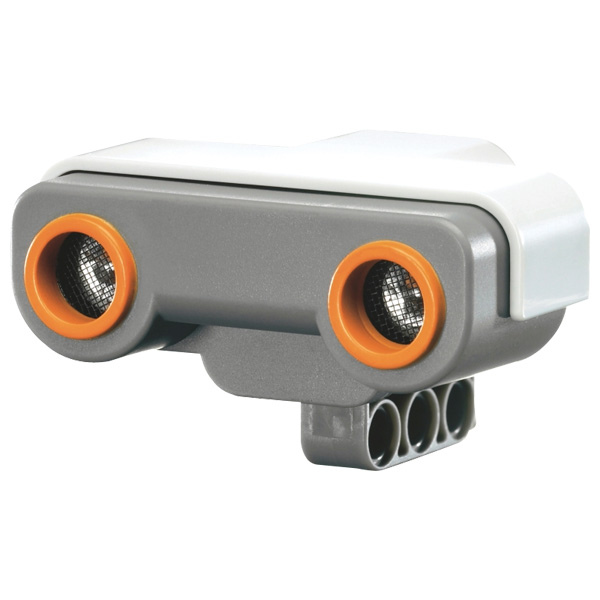
\includegraphics[width=110px, clip=true, trim = 0px 90px 0px 0px]{sensor/us}
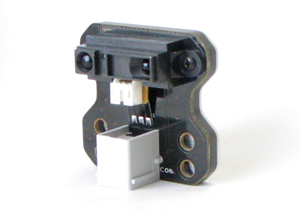
\includegraphics[width=110px]{sensor/infrared_sensor}
\begin{itemize}
\item Begge har en afvigelse på $\pm$ 3 cm
\item Den ultrasoniske sensor har en range på 20-170 cm
\item Den infrarøde sensor har en range på 10-56 cm
\end{itemize}
\end{frame}
\begin{frame}
\frametitle{Valgt motor}
\center
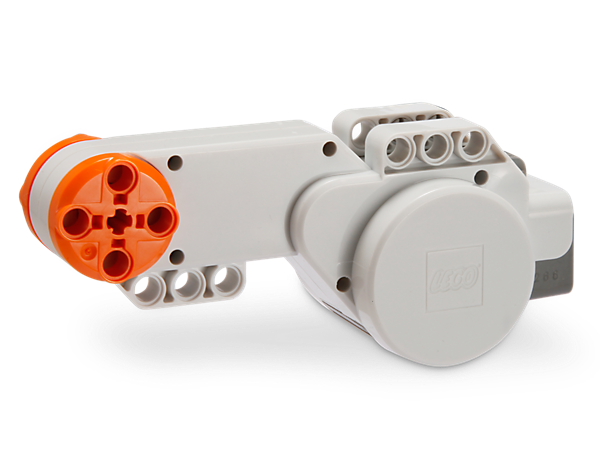
\includegraphics[width=110px]{sensor/lego_motor}
\begin{itemize}
\item Store afvigelser i testen på op til +7 og -4 grader
\item Lokaliseringen skal afhjælpe upræcisionen
\end{itemize}
\end{frame}
\subsection{Lokalisering}
\begin{frame}
\frametitle{Valg af Kinect}
\begin{itemize}
\item Nem tilslutning til PC
\item Mange sensorer
\item Gode udviklingsværktøjer
\item Tilgængelig gennem universitetet
\end{itemize}
\end{frame}
\subsection{Mapping}
\begin{frame}
\frametitle{Occupancy grid}
\begin{itemize}
\item Til at kortlægge har vi valgt at bruge \textit{occupancy grid} algoritmen
\item \textit{Occupancy grid} er en familie af algoritmer som gør det muligt at generere konsistente kort
\item \textit{Occupancy grid} opdeler kortet i celler og tildeler en binær tilfældig variabel til hver celle
\end{itemize}
\end{frame}